\lecture{1}{Sat 23 Sep 2023 16:28}{}

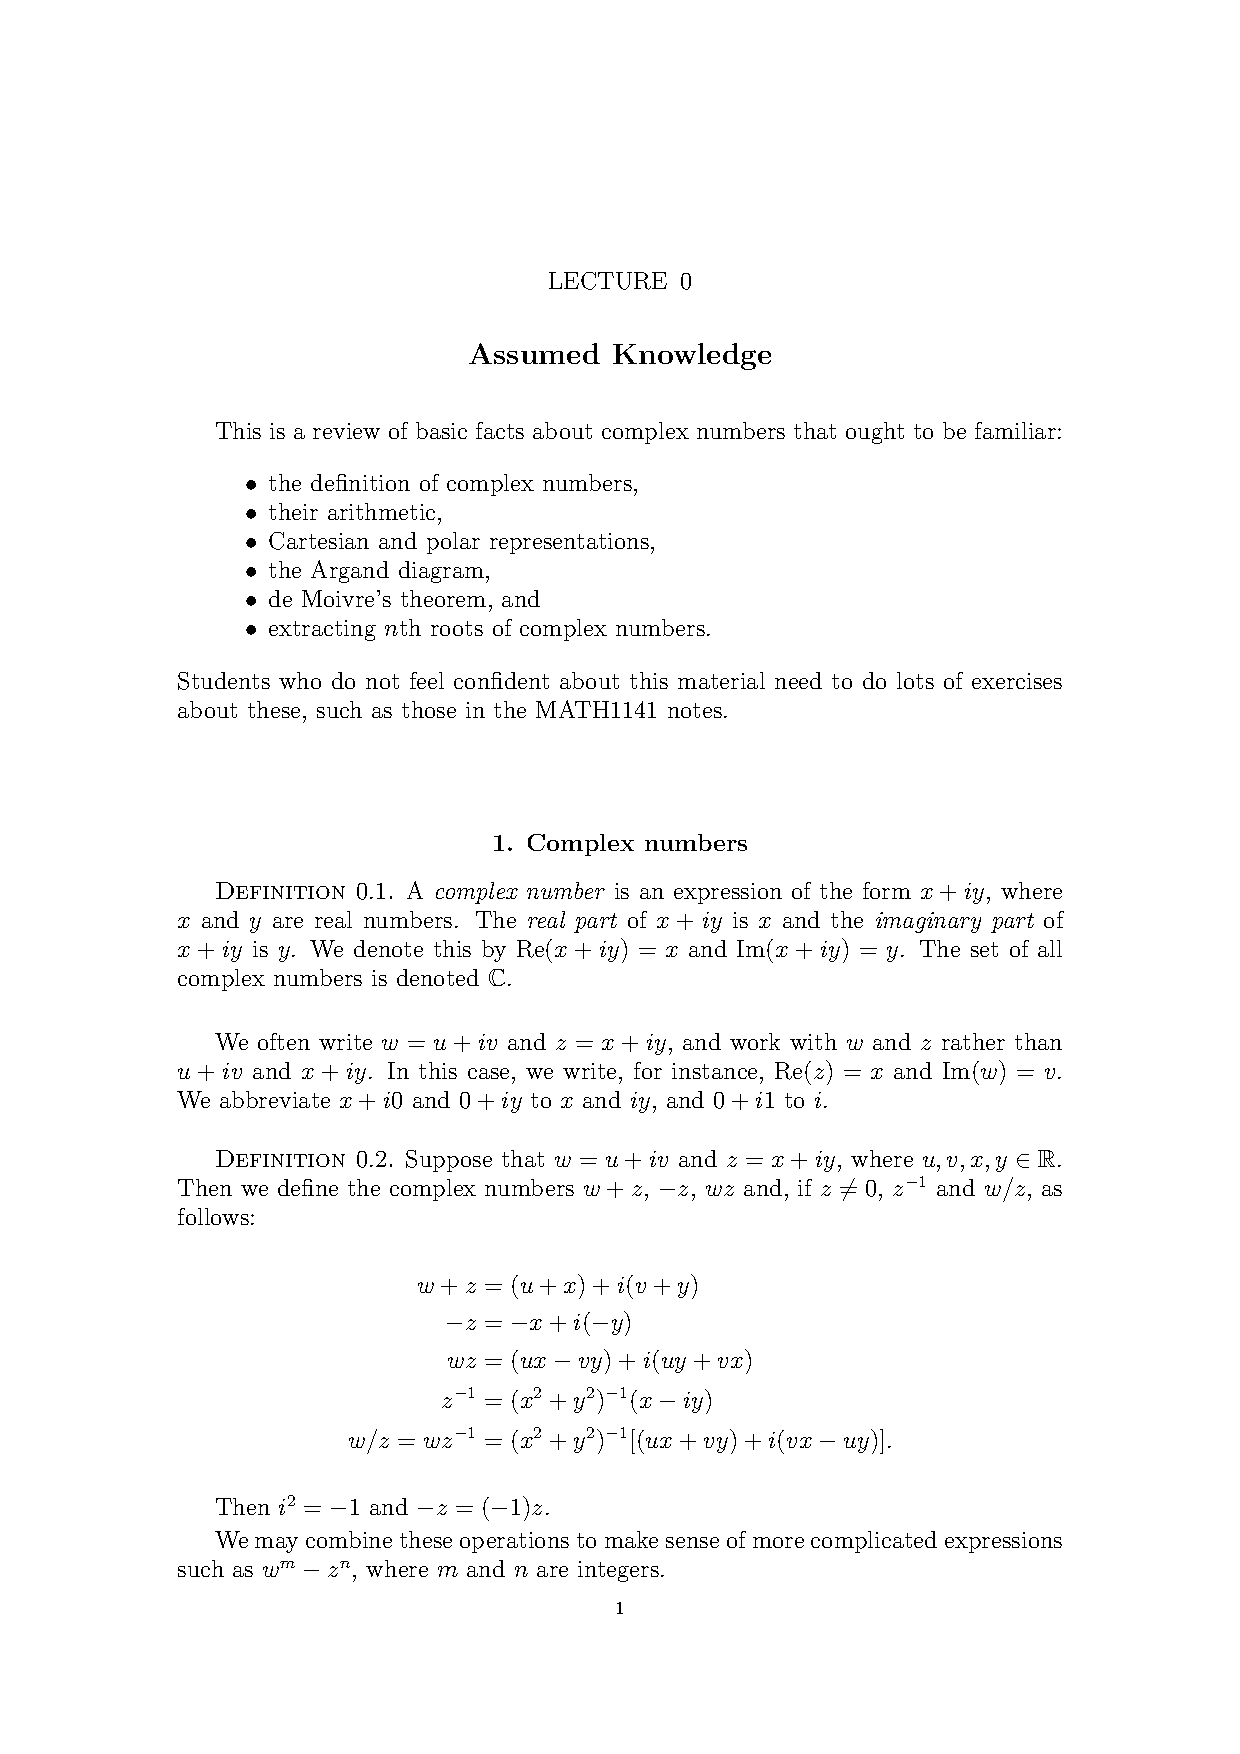
\includepdf[pages=1-16]{notes-2022.pdf}
Exercise 2.13:
We can set \( w = u + iv. \) If \( z \) is on the line \( x=1 \), then \( Re(z ) = 1\),
whence \( Re(\frac{1}{w}) = 1 \) (and \( w \neq 0 \)). Now
\begin{align*}
  1 = Re(\frac{\overline{w}}{\mid w\mid^2}  )=\frac{u}{v^2 + u^2}
.\end{align*}

It follows that \(u^2 + v^2 = u \), whence \( (u-\frac{1}{2})^2 + v_{2} = \frac{1}{4} \), and the result follows
we can reverse this mapping and show that every point on the circle except 0 arises this way. Thus the image of the line is the
circle with the point 0 removed.




